
En este capítulo se detalla la implementación del compilador
y la máquina virtual diseñadas para utilizar el lenguaje
\frob{} en la plataforma elegida.
También se explica cuál sería el mecanismo para portar la
implementación a otra plataforma.

%TODO: Completar la intro luego de tener los caps.

\section{Compilador}

  El compilador será el encargado de leer el programa \frob{} y traducirlo
a \alf{}.

  El lenguaje utilizado para desarrollar el compilador fue \textit{Haskell}.
  Las razones que llevaron a su elección son la portabilidad y la
expresividad del mismo.
  El compilador \compilador{} es portable, ya que se puede compilar y ejecutar
en diversos sistemas operativos utilizando el compilador \textit{ghc}.

  Es usual realizar tareas de compilación en \textit{Haskell} por lo que existen
herramientas estándar para cada etapa.

  El compilador constará de una secuencia de etapas: Análisis Léxico,
  Análisis Sintáctico, Análisis Semántico y Generación de Código.

  En la Figura \ref{fig:compiler} se puede ver la estructura más detallada
del compilador.

\begin{figure}[h!]
\begin{center}
\caption{Diagrama del compilador}
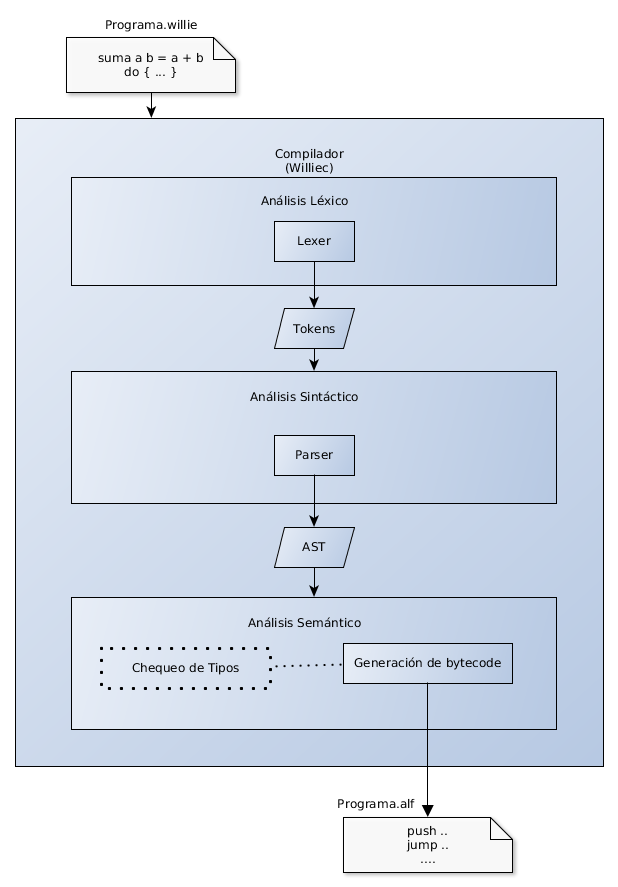
\includegraphics[width=0.9\textwidth]{graphs/compiler.png}
\label{fig:compiler}
\end{center}
\end{figure}


\subsubsection{Análisis Léxico}
  La primera etapa se llama análisis léxico, en esta se lee el código
  fuente en lenguaje \frob{} (.willie) y lo transforma en una
  lista de lexemas.

  Un lexema puede ser una palabra reservada (ej: \texttt{do}),
  un valor (ej: $19$), un identificador (eg: \texttt{distance}) o un símbolo reservado (eg: \texttt{+}).

  Para representar los lexemas, se utiliza la herramienta \textit{UU.Scanner}
  \cite{uuparser} que estandariza los mismos en el tipo de
  datos \texttt{Token}.
  Usando \textit{Alex} se procesa el código fuente, se reconocen los lexemas y se retorna una lista de tipo \texttt{[Token]}.

  La etapa se puede resumir en la implementación de la función \texttt{tokenize}.

\begin{Verbatim}
  tokenize :: String -> String -> [Token]
\end{Verbatim}




\subsubsection{Análisis Sintáctico}
  La segunda fase del compilador, recibe la lista de lexemas (\texttt{[Token]}) y
reconoce el lenguaje, generando un árbol de
sintaxis abstracta (\emph{AST}\footnote{Del inglés Abstract Syntax Tree}).

  Para reconocer la gramática se implementó un parser recursivo descendente.
  Utilizando la herramienta \textit{UU.Parser} \cite{uuparser}, se definió un tipo de datos
  \texttt{TokenParser a} que representa un parser que recibe una secuencia de lexemas de tipo \texttt{Token}
  y retorna un \emph{AST} de tipo \texttt{a}.

  \begin{Verbatim}
  type TokenParser a = Parser Token a
  \end{Verbatim}

  \textit{UU.Parser} define un conjunto de combinadores de parsers y utilizándolos se construyen parsers
  complejos a partir de parsers simples.

  Para representar el \emph{AST} se utiliza una gramática de atributos.
  Una gramática de atributos es como una gramática libre de contexto, pero agrega semántica a la misma.
  Para el análisis sintáctico, la semántica no es utilizada, pero será usada en la próxima etapa.

  El sistema de gramáticas de atributos
  \textit{UUAG}\cite{uuag} fue usado para la implementación.


  Se define un tipo de datos \texttt{Root} que representa la raíz del árbol.

  \begin{Verbatim}
  data Root
    | Root
      decls :: Decls
      dodecls :: Dodecls
  \end{Verbatim}

  El mismo tiene un único constructor \texttt{Root\_Root} que recibe un árbol de tipo
  \texttt{Decls} que representa las declaraciones, y un árbol de tipo \texttt{Dodecls} que
  representa el bloque \texttt{do}.

  Para crear el \emph{AST} usando \textit{UU.Parser} se define el parser \texttt{pRoot}:

  \begin{Verbatim}
  pRoot :: TokenParser Root
  pRoot
    = Root_Root <$> pDecls <*> pDodecls
  \end{Verbatim}

  El cuál asume definido un parser de declaraciones \texttt{pDecls} y un parser
  del bloque \texttt{do} (\texttt{pDodecls}).
  
  \begin{Verbatim}
  pDecls :: TokenParser Decls

  pDodecls :: TokenParser Dodecls
  \end{Verbatim}

  El combinador ``$\langle * \rangle$'' \cite{uuparsing:piriapolis} se utiliza para
  combinar dos parser y resolver producciones de largo 2 en una gramática,
  en este caso reconocer primero la lista de declaraciones de funciones, y
  luego el bloque \texttt{do}.
  El tipo del combinador es:

  \begin{center}
    $(\langle*\rangle) :: \texttt{Parser}\ s\ a \rightarrow \texttt{Parser}\ s\ b \rightarrow \texttt{Parser}\ s\ (a, b)$
  \end{center}

  El combinador ``$\langle \$ \rangle$'' se utiliza para aplicar una
función al resultado de un parser, en éste caso la función es aplicar
el constructor \texttt{Root\_Root}.

  Para construir el parser completo, se va refinando sucesivamente
en parsers mas específicos, hasta construir completamente el \emph{AST}.
  En el apéndice \ref{appendix:parser} se encuentra código del parser
implementado.



\subsubsection{Análisis Semántico}
  Para la última etapa se utiliza la gramática de atributos para definir
semántica sobre el \emph{AST}.

Las gramáticas de atributos (\emph{Attribute Grammars}
\cite{attributegrammars} \cite{uuag}) simplifican
la tarea de escribir catamorfismos.
Un catamorfismo es una función análoga a la función de alto orden
\texttt{foldr} pero aplicada sobre cualquier tipo de datos recursivo.

  De ésta manera se pueden definir atributos sintetizados,
  heredados o mixtos en el \emph{AST}.

  Los atributos sintetizados son valores que se distribuyen desde las
hojas hacia la raiz del \emph{AST}, y los heredados aquellos que
se distribuyen desde la raiz hacia las hojas.

  Uno de dichos atributos será el código en bajo nivel, la salida
de esta etapa.

  Se implementó una gramática de atributos usando \textit{UUAG}, y con
  el compilador de gramáticas \textit{UUAGC}\cite{uuagc} se
  compiló a \haskell{}.

  El compilador \textit{UUAGC} toma la gramática y construye los
  catamorfismos necesarios para procesar todos los atributos.

  Construir el compilador, se reduce a obtener una secuencia de atributos
  sobre el \textit{AST} que sirven para generar el código \alf{}.

  Por ejemplo para construir el código de un programa, la raiz
  del \textit{AST} está dada por el tipo de datos \texttt{Root}.

\begin{Verbatim}
data Root
  | Root
      decls :: Decls
      dodecls :: Dodecls
\end{Verbatim}

  Se puede definir el código como la concatenación del código de
  las declaraciones del bloque \texttt{do}, una instrucción \texttt{halt}
  y el código de las declaraciones de funciones (\texttt{Decls}).

  Para ésto se define un atributo sintetizado (\texttt{syn})
  llamado \texttt{code}.


\begin{Verbatim}
set All = Root Decls Decl Dodecls Dodecl Expr
attr All syn code use {++} {[]} :: BC

sem Root
  | Root
    lhs.code = @dodecls.code ++ [Thalt] ++ @decls.code
\end{Verbatim}

  Utilizando la palabra clave \texttt{Set} se define el conjunto \texttt{All}
de elementos para los que se definirá el atributo.
  
  En la definición del atributo, se especifica que en caso de no haber
una regla específica, se calcula usando la concatenación \texttt{++}
y como atributo por defecto toma \texttt{[]}. A ésto se le llama
\textit{use rule}.

  \begin{Verbatim}
  attr All syn code use {++} {[]} :: BC
  \end{Verbatim}

  Por ejemplo para la definición de la lista de declaraciones:

\begin{Verbatim}
type Decls = [Decl]
\end{Verbatim}

  No es necesario especificar que el código se obtiene concatenando sus
  partes ya que se infiere automáticamente usando la regla anterior.


  Para poder generar el código de todo el programa, es necesario
  calcular otros atributos previos.
  Se necesita saber la posición en la que quedarán las funciones para
  poder tener una referencia a ellas.
  Para saber la posición, es necesario calcular el largo del código
  antes de tener el código.

  Para ésto se definió un atributo sintetizado \texttt{len} que contiene
  el largo que tendrá cada bloque luego de traducido
  a código, pero sin llegar a traducirlo.

  También se definió un atributo \texttt{pos} que indica en que posición
  estará ubicado el código que se genere para cada producción de la
  gramática.
  El atributo \texttt{pos} es un atributo heredado (\texttt{inh}) en
  el \textit{AST}.

  Por ejemplo en \texttt{Root}, se utiliza el atributo \texttt{len} 
  de las declaraciones del bloque \texttt{do} para saber a partir
  de que posición \texttt{pos} estarán ubicadas las declaraciones
  de funciones.

\begin{Verbatim}
attr All syn code use {++} {[]} :: BC
         syn len use {+} {0} :: Int
         inh pos :: Int
 
sem Root
  | Root
      lhs.code = @dodecls.code ++ [Thalt] ++ @decls.code
      dodecls.pos = 0
      decls.pos = @dodecls.len + 1
\end{Verbatim}

  Utilizando el atributo \texttt{pos}, se puede saber en que posición
  estará cada función en el código generado.
  Para tener la posición de todas las funciones se utiliza un atributo
  encadenado (\texttt{chn}) llamado \texttt{labels},
  es heredado pero también es sintetizado.
  Por ejemplo al declarar una función, se agrega la posición \texttt{pos}
  asociada al nombre de la misma.

\begin{Verbatim}
sem Decl
  | Function
      lhs.code = @body.code ++ [Tret]
      lhs.len = @body.len + 1
      lhs.labels = addLabel @name @lhs.pos @lhs.labels
\end{Verbatim}

  El atributo contiene un mapa que dado un nombre de una función retorna
  la posición de la misma, \texttt{labels} recolecta la posición de todas
  las funciones.
  Luego otro atributo \texttt{labelMap} se declara como heredado \texttt{inh}
  y se le asigna en \texttt{Root} el valor de \texttt{labels},
  \texttt{labelMap} se usa para distribuir el mapa
  completo en todo el \textit{AST}.

\begin{Verbatim}
sem Root
  | Root
      decls.labels = emptyLabelMap
      decls.labelMap = @decls.labels
      dodecls.labelMap = @decls.labels
\end{Verbatim}

  Por último un atributo \texttt{env} encadenado recolecta las declaraciones
  de identificadores, a cada identificador de señal le asigna un número
  entero único y mantiene la lista de las variables en el alcance (scope)
  dentro de una función. 
  Luego que el atributo \texttt{env} recolecta todas las declaraciones,
  el resultado es distribuido con el atributo heredado \texttt{envInh}.

\begin{Verbatim}
sem Root
  | Root
      decls.env = emptyEnv
      dodecls.env = emptyEnv
      dodecls.envInh = @dodecls.env
\end{Verbatim}

  Usando todos éstos atributos se genera el código para cada producción
  de la gramática, y el atributo \texttt{code} se puede calcular.

  Se definió un módulo \texttt{Bytecode} que abstrae el código
  de máquina en un tipo \texttt{OpCode} y define funciones para 
  exportarlo como texto o en formato binario.

% TODO(Marcos): Agregar un diagrama con los modulos, indicando que es
% generado y que importa a que.

  Al compilar la gramática usando \textit{UUAGC} se obtiene un módulo
  en lenguaje \texttt{Haskell} que expone la función \texttt{code\_Syn\_Root}
  y deja accesible el código resultado como una lista de
  tipo \texttt{[OpCode]}.

  Utilizando el módulo \texttt{Bytecode}, el código se obtiene y 
  escribe en un archivo (.alf) terminando el proceso de compilación.



\section{Máquina virtual}
  
  
  La máquina virtual será la encargada de recibir el bytecode creado por
el compilador, e interpretarlo en la plataforma que esté ejecutando.
  A diferencia del compilador, es necesario implementar una máquina virtual
para cada arquitectura objetivo.\\

  Por ejemplo, para ejecutar programas en un robot
  con un procesador \emph{arduino}, debe
  existir una implementación de la máquina para ese modelo
  de \emph{arduino}.

  Al momento de implementar la máquina, se tomará en cuenta ésto para
  factorizar partes en común y sólo implementar por arquitectura, las
  partes que realmente sean diferentes como ser la comunicación con
  los periféricos de entrada/salida y las llamadas al sistema.


TODO: Describir el diseño de la máquina virtual.

  La máquina virtual va a ser basada en stack. Ésto significa
que las operaciones van a tomar sus argumentos del stack y
colocar resultados en el mismo.

